\section{Problem statement}
\label{subsec:problemStatement}

The goal with this research is to optimize urban transit networks in order to increase the number of public transportation passengers. As mentioned, the current solution of Trondheim' transit network consist of an experience based route network. This means the transit routes are not properly, computationally optimized concerning the travel demand and travel time. In order to contribute to this, we will in this thesis create a swarm intelligence inspired algorithm for the UTRP. A good route network will ensure that routes having the most traveling demands are satisfied with short paths and few vehicle transfers, making travel demand a key variable for the algorithm. AtB\citep{website:atb} does not possess accurate data about the travel demand, and detailed investigations into measuring and predicting travel demand is a complex research problem, beyond the scope of this thesis. Demand values and travel times are all provided for Mandl's benchmark problem\citep{mandl79}. For the UTRP, Mandl's benchmark problem is widely used, whereas a recognized metric is established for evaluating the performance. Mandl's benchmark problem will therefore be used as the input data for most of the experiments in this thesis. Acknowledged performance criteria will be used to determine the performance of the algorithm and comparing the results with approaches published in the literature\citep{nikolic14,kechagiopoulos14,mandl79,kidwai98, fan10, chakroborty02, zhang10, chew12}.

The classical ACO has several advantages for VRP, such as natural parallelism and continuous positive feedback, which allows good solutions to be identified fast. However, ACO also has a few shortcomings which includes the weakness of getting stuck at a local optima. We will investigate the possibility of overcoming this drawback and to enhance the optimization process by improving ACO. Changes to the classic ACO has previously been done to overcome some of the algorithm's known weaknesses. Giving the ants knowledge of the visited nodes\citep{sedighpour14,salehinejad10,poorzahedy11}, and adding a notion of the best known solution so far\citep{tripathi09,sedighpour14} showed improved performance. PSO and BCO use related approaches for rewarding the global best solution so far, and \citet{kechagiopoulos14} and \citet{nikolic14} demonstrates good performance with their respective PSO and BCO implementations. In order to answer \vref{itm:RQ2}, we will investigate whether incorporating additional features with respect to how PSO and BCO operates will improve the ACO performance further.

\vref{itm:RQ3} is concerned whether the implementation can be used to optimize real urban transit networks. This cannot be fully answered until it is applied to a real city, but we will strive to create a method that is easily adaptable with the concerns of public transportation in cities in mind. Real urban cities are (often) a whole lot larger than Mandl's relatively small network (Fig. \vref{fig:MandlNetwork_problemstatement}). To  test whether it is possible to apply the proposed algorithm in large urban cities, the algorithm will be implemented in a way that it is easily adaptable to new input values, and it will be tested on large networks more similar to real transit networks. 

As mentioned in Section \vref{subsec:relatedWorkConclusion} will we investigate how the usage of a Neo4j database affects our development process and the quality of the solution. In order to do this will the networks be represented as Nodes and Relationships in a Neo4j database, and the generated routes will also be added to the database. We will also strive to use the built-in methods in Neo4j in order to establish their usability in solving UTRPs with a swarm intelligence inspired system. 

%\subsubsection*{RQ 2: Is it efficient to add attributes from other swarm intelligence-methods in order to improve the ant colony optimization algorithm?}

%\subsubsection*{RQ 3: Is it possible to apply the proposed algorithm to optimize urban transit routes in large urban cities?}

\begin{figure}[H]
\begin{center}
  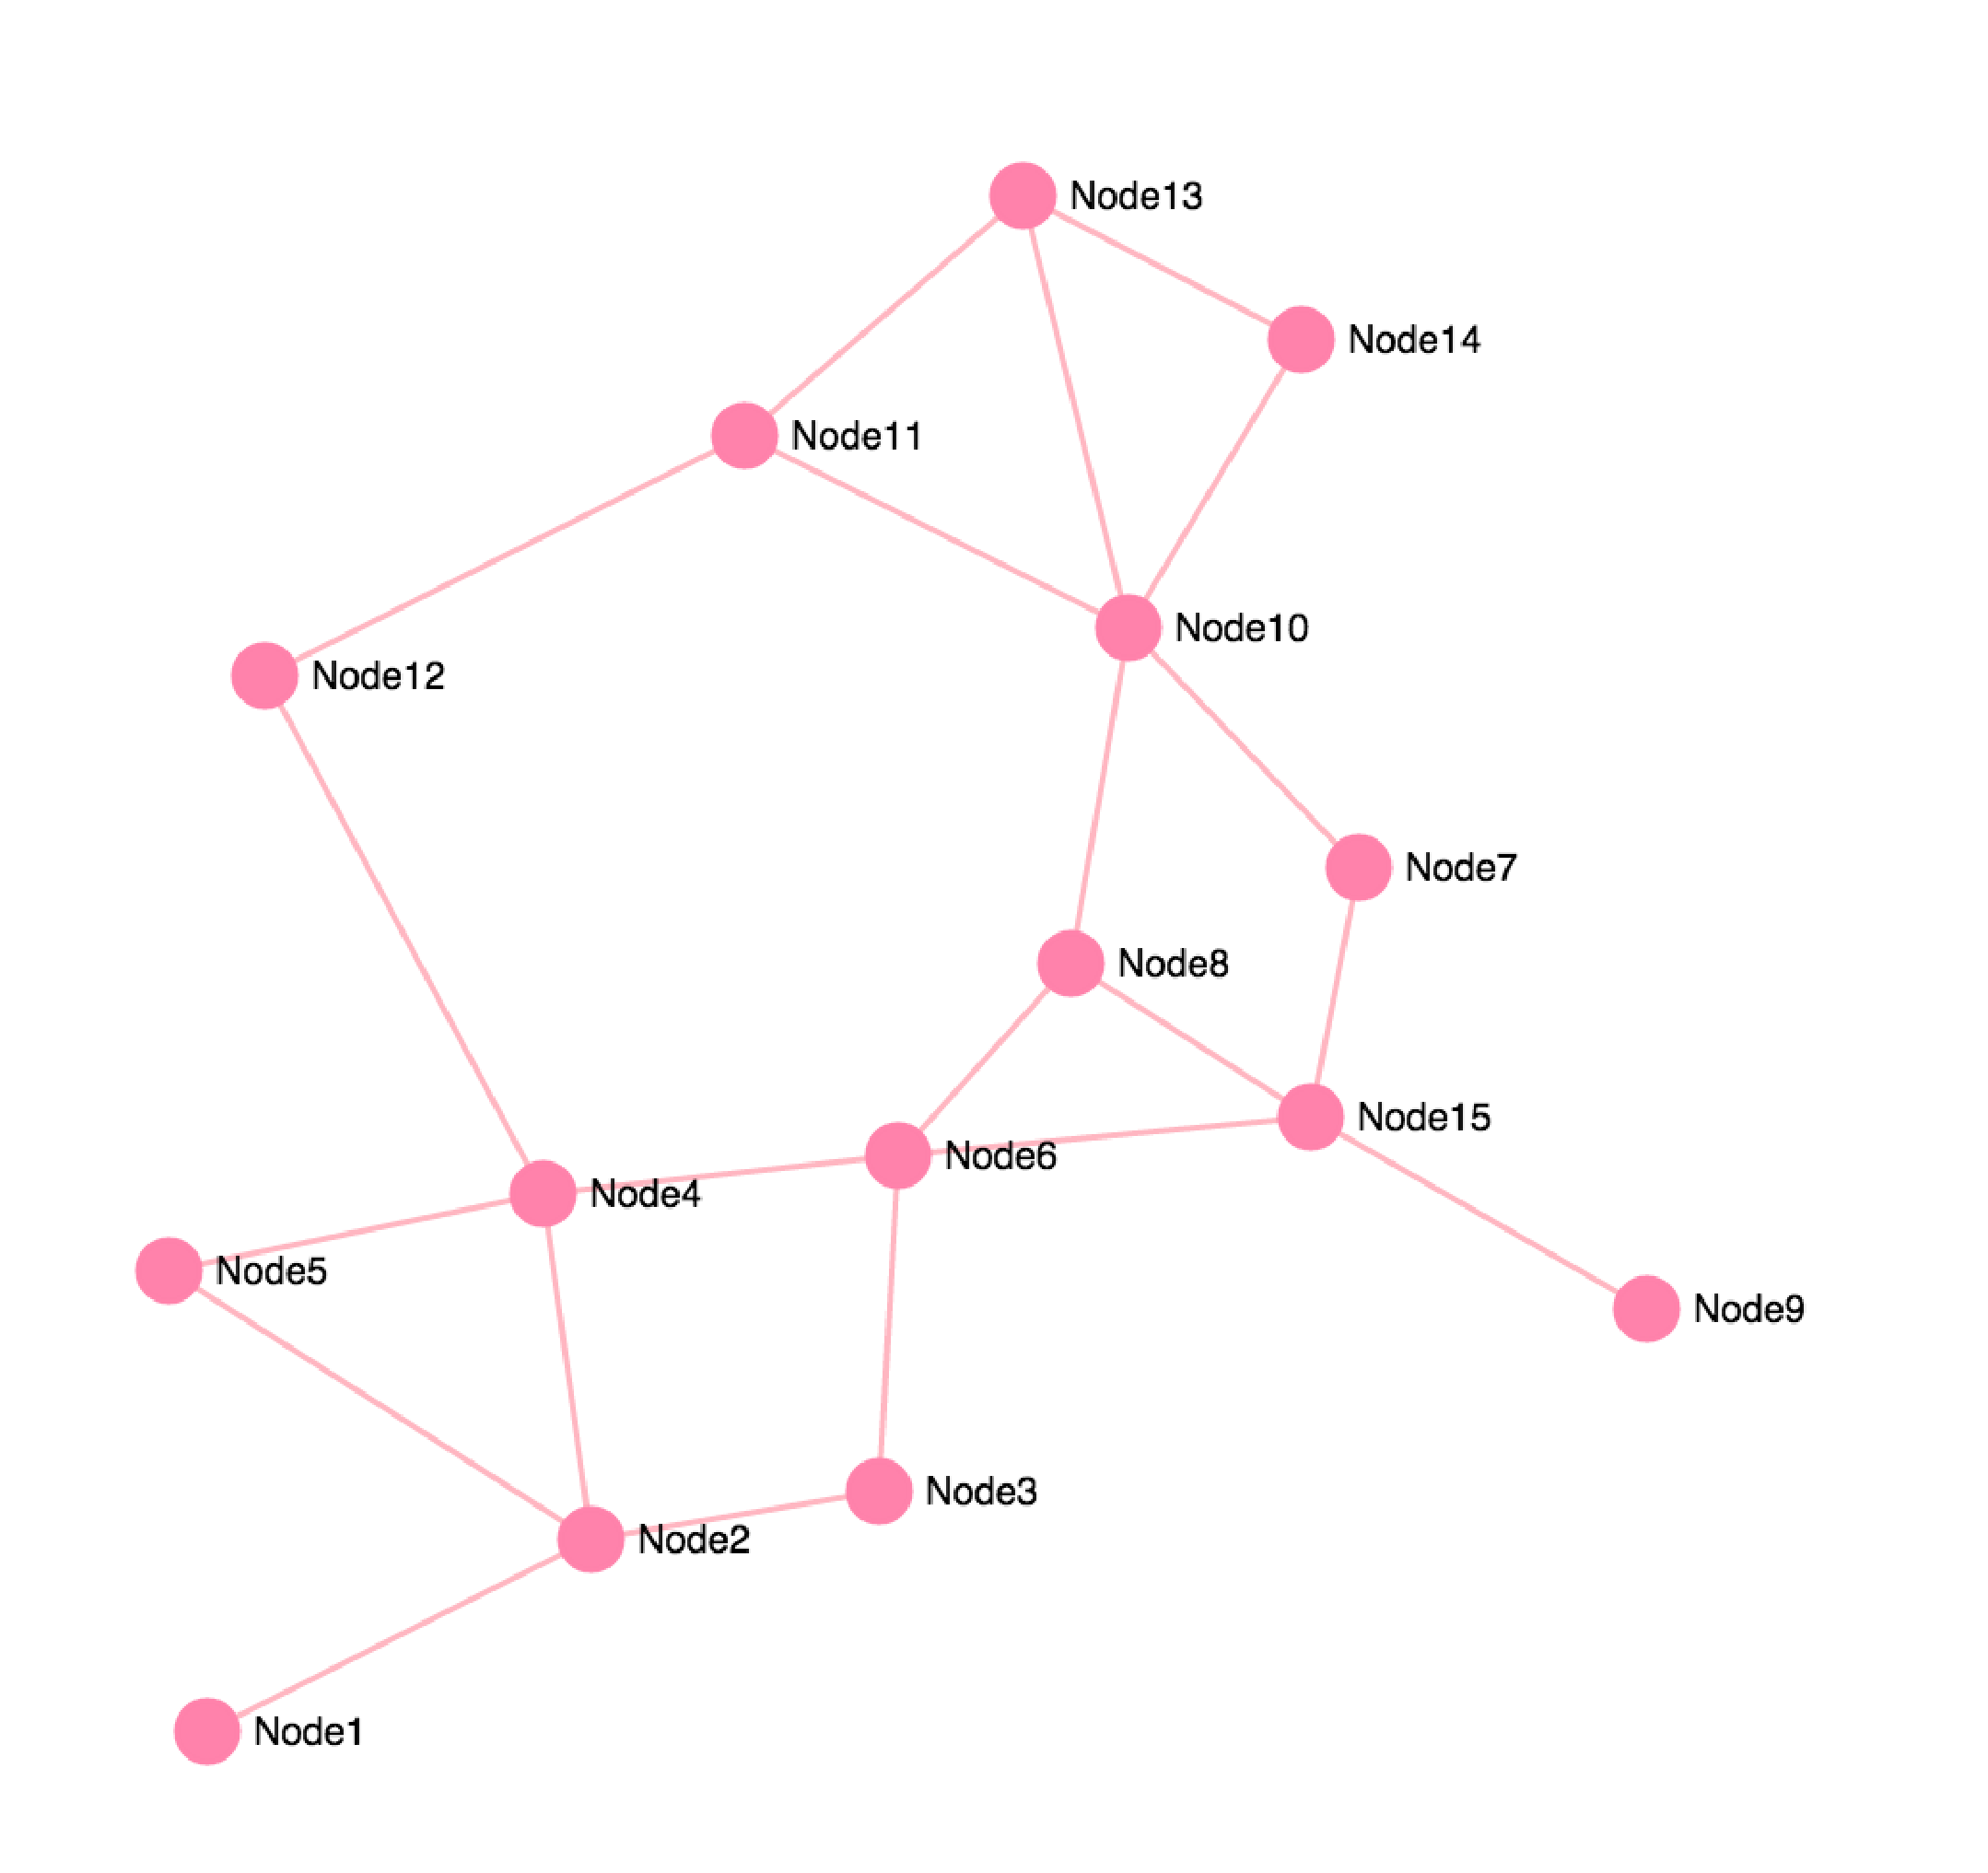
\includegraphics[width=4in]{assets/mandlnetwork_crop.png}
  \end{center}
  \caption{Illustration of Mandl's transit network as a graph}
  \label{fig:MandlNetwork_problemstatement} 
\end{figure}







